\documentclass[12pt,a4paper]{article}
\usepackage[a4paper, margin=1.5cm]{geometry}
\usepackage{graphicx}
\graphicspath{{./images/}}
\usepackage{subcaption}
\newcommand{\tr}{\mathrm{tr}}
\usepackage{hyperref}
\usepackage{authblk}
\usepackage[backend=biber,style=nature]{biblatex}

\bibliography{article}
\addbibresource{article.bib}


\begin{document}
\title{Ionizations of Liquid Water from Charged-cell Periodic Subsystem DFT and Embedded Coupled Cluster Simulations}
\author[1]{Jessica Martinez}
\author[1]{Pablo Ramos}
\affil[1]{Department of Chemistry, Rutgers University, Newark, New Jersey}
\author[2]{Andre Gomes}
\affil[2]{Université de Lille, CNRS, UMR 8523 – PhLAM – Physique des Lasers, Atomes et Molécules, Lille, France}
\author[3]{Johannes Tölle}
\affil[3]{Theoretische Organische Chemie, OrganischChemisches Institut and Center for Multiscale Theory and Computation (CMTC), Westfälische Wilhelms-Universität Münster, Corrensstraße 40, 48149, Münster, Germany}
\author[1]{Michele Pavanello}
\date{}
\setcounter{Maxaffil}{0}
\renewcommand\Affilfont{\itshape\small}
\begin{titlepage}
  \maketitle
\end{titlepage}

\begin{abstract}
Modeling the ionization potential (IP) and electron affinity (EA) of liquid water is challenging for
two reasons: (1) the bulk-like nature of the liquid imposes the use of periodic boundary conditions
(PBCs), which pose roadblocks when considering charge systems; (2) quantitative electronic structure
methods, such as coupled cluster, are generally not available in PBCs. In this work, we tackle both
challenges by employing subsystem DFT to split the extended system into a collection of finite
subsystems embedded by extended, infinite subsystems. This is achieved by an impurity
model ~\cite{tolle2019charged} where coupled cluster wavefunctions can be introduced to evaluate
the water molecules’ energy functionals. 

The liquid’s electronic structure is expressed in subsystem contributions by invoking nonadditive density 
functionals whereby the total energy of the liquid is expressed as the sum of molecule-additive
and nonadditive contributions ~\cite{martyna1999reciprocal}. The inter-molecular interaction is
split into Coulumb interactions, and such nonadditive terms as the noninteracting
kinetic energy and the noninteracting exchange-correlation ~\cite{krishtal2015subsystem}. 
These contributions represent interactions related among others to exchange, van der Waals and
Pauli repulsion and are all bifunctional of the subsystem densities ~\cite{tolle2019charged}. 

Embedding potentials are computed with the embedded Quantum ESPRESSO (eQE) ~\cite{genova2017eqe} 
software employing ultrasoft pseudopotentials. The ground state calculation of each subsystem with
the corresponding neutral and polarized embedding potential was carried out with 
DIRAC ~\cite{saue2020dirac} and ADF ~\cite{te2001chemistry}. The final IP/EA values reproduce the
experimental values to within 0.5 eV and are determined averaging over 256 water molecules
(or subsystems) considered in the simulation cell, calculated by the energy difference of the
neutral and the polarized system (Called SCF method) ~\cite{bagus1965self,waskom2017mwaskom}. 
\end{abstract}


\section{Introduction}

\section{Theoretical Background}

\subsection{Mapping a periodic system into a collection of non-periodic subsystems and one periodic subsystem}
To cast DFT in a subsystem fashion, we invoke nonadditive functionals in which each energy term of the supersystem is expressed as the sum of additive
and nonadditive contributions ~\cite{martyna1999reciprocal}. Therefore, when dealing with a finite subsystem with electron density $\eta_I$, and an
infinite or extended subsystem with electron density $\eta$ - $\eta_I$, the total energy is given by,

\begin{equation}
	E_{tot} = {E_[{\eta}_I]} + {E_[{\eta} - {\eta}_I]} + {E^{int}[{\eta}_I, {\eta} - {\eta}_I] } 
\end{equation}

And the interaction energy can be broken down into the following contributions,

\begin{equation}
	E^{int} = E^{int}_H + V^{int}_eN + T^{nad}_s + E^{nad}_{xc} 
\end{equation}

The two Coulombic terms $E^{int}_H$ and $V^{int}_eN$ are the electron-electron and electro-nuclear interactions, respectively. And the
nonadditive terms $T^{nad}_s$ and $E^{nad}_{xc}$, represent the noninteracting kinetic energy of the system and the noninteracting
exchange-correlation functionals, respectively ~\cite{krishtal2015subsystem}. The two last terms represent interactions related among other to exchange, van der Waals and Pauli repulsion and are all bifunctional of the two subsystem densities.

\subsection{Neutral System Coulomb interaction energy determination}

For the neutral system, the Coulomb interaction energy can be expressed as a potential that maps the interaction of an accurately infinitely extended
environment onto and isolated subsystem $I$,

\begin{equation}
	v^{'}_{int} [\eta] (r) = v[\eta](r) - \bar{v} {\eta_I}(r)
\end{equation}

Where $v[\eta](r)$ is the total Coulomb potential of the system and $\bar{v} {\eta_I}(r)$ the potential of the isolated subsystem $I$.

\subsection{Embedding potential scheme}
\subsection{Impurity Model}
\section{Computational Section}

\section{Results}
\subsection{IPs of Bulk water}

\begin{figure}[!h]
	\captionsetup[subfigure]{labelformat=empty}
	\centering
	\begin{subfigure}{0.4\linewidth}
		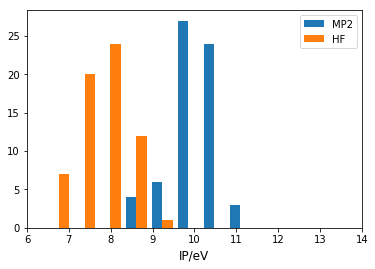
\includegraphics[width=\linewidth]{IP-mp2-hf}
		\caption{MP2 vs HF}
	\end{subfigure}
	\begin{subfigure}{0.4\linewidth}
		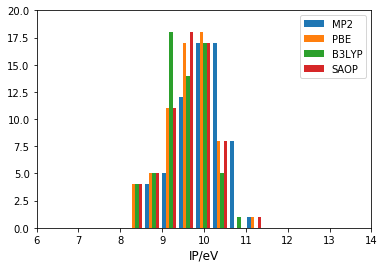
\includegraphics[width=\linewidth]{IP-mp2-dft}
		\caption{MP2 vs DFT}
	\end{subfigure}
	\caption{Distribution of IPs of bulk liquid water. The area subtenended by the lines sums up to 64(ie, the number of subsystems). Left: Comparison between MP2 and HF. Right: Comparison between MP2 and DFT}
\end{figure}

\begin{table}[!h]
 \begin{center}
  \caption{average IPs}
  \label{tab:table1}
  \begin{tabular}{ |c|c| }
	\hline\hline
	&IP average (eV)\\
	\hline
	MP2&9.9941\\
	\hline
	HF& 7.8250\\
	\hline
	PBE&9.6089\\
        \hline
        B3LYP&9.5147\\
        \hline
        SAOP&9.5897\\
	\hline
   \end{tabular}
 \end{center}
\end{table}

\section{Conclusions}

\nocite{*}

\printbibliography

\section{Acknowledgments}


\end{document}
